\chapter{Planeaci\'on}
\section{Planeaci\'on Organizacional}
\subsection{Misi\'on}
Ser l\'ideres en la satisfacci\'on de las necesidades del consumidor con alimentos saludables, con atributos de confianza, cercan\'ia y valor agregado; con responsabilidad frente a los accionistas, colaboradores, empleados, cliente, medio ambiente y a la sociedad..%
\\%
\\%
Hornitos S.A. se proyecta con ser  una corporaci\'on de negocios con varias sucursales en las diferentes ciudades de  Colombia. Y en las principales de Am\'erica tratando de mostrarnos en el mercado internacional como una gran potencia en la econom\'ia Colombiana.
\\%
\\%
Buscaremos consolidarnos como una gran empresa que siempre va a estar comprometida con su comunidad es decir siempre va pensar en sus clientes y consumidores primero para asi lograr su fidelidad y preferencia.
\\%
\\%
tendremos el mejor personal capacitado constantemente que se especializa en el buen trato de los clientes, adem\'as de esto Hornitos S.A compromiso con el medio ambiente nos caracteriza por la eficiencia de nuestros procesos y la continua actualizaci\'on tecnol\'ogica de nuestras plantas por medio de la utilizaci\'on de nuestras tecnolog\'ia afianzaremos nuestro producto en el mercado nacional y generaremos cada ves mas empleos al expandir nuestra industria.
%
\subsection{Visi\'on}
Compa\~n\'ia la cual ser\'a reconocida por su liderazgo, competitividad e innovaci\'on, cuyos productos y servicios son la opci\'on preferida del consumidor colombiano, con participaci\'on destacada en la comunidad latinoamericana y presencia en otros mercados.
\\%
\\%
Hornitos S.A ser\'a l\'ider en distribuci\'on y tendr\'a los mas altos m\'argenes de ventas en colombia y una excelente presencia en las principales ciudades del mercado internacional y nos destacaremos por la efectividad de nuestro mercadeo por la calidad de nuestros productos como la mejor fuente de empleo por nuestra responsabilidad social.
\section{Plan estr\'ategico de ventas}
\begin{figure}[htbp]
%centering es para centrar la imagen
	\centering
%aca es donde se incluye la imagen, se da el ancho(width), \textwidth significa que con repescto al tamano del
%texto y luego la ruta, relativa siempre es decir, a partir de donde se esta, como images esta ahi
%dentro, solo se usa desde images y ojala nada de espacios en el nombre de la imagen
		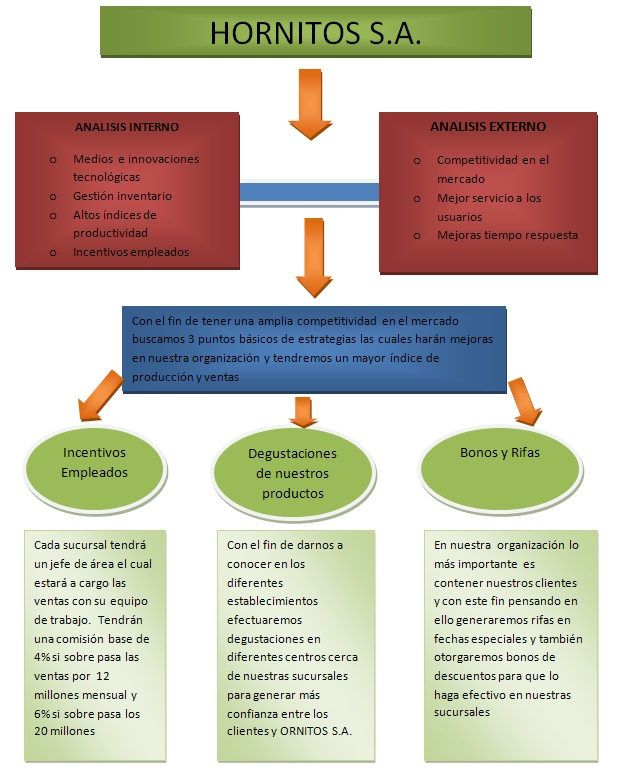
\includegraphics[width=0.60\textwidth]{images/Dibujo.jpg}
%el caption es para el texto que aparece debajo de la imagen
	\caption{Plan estrategico}
%label es para darle una referencia, por ejemplo si uno dice "como se puede ver en la imagen a1"
	\label{fig:Plan estrategico}
\end{figure}%
Hornitos S.A. Ha desarrollado una campa\~na la cual se dividir\'a en 3 partes las cuales buscara tener  por medio de los clientes una preferencia en nuestros productos e incentivar a nuestros trabajadores a tener mayor entrega con la organizaci\'on estar\'iamos hablando de tres proyectos los cuales buscaran un mejor \'ambito para la organizaci\'on.%
\\%
	
	\begin{itemize}
		\item Incentivos empleados.
		\item Degustaciones.
		\item bonos y rifas.
	\end{itemize}
	
\subsection{Incentivos empleados:}Cada sucursal tendr\'a un jefe de \'area el cual estar\'a a cargo las ventas con su  respectivo equipo de trabajo.  Tendr\'an una comisi\'on base de ventas pero con un incentivo adicional para los trabajadores y el jefe de la sucursal si logra sobre pasar ventas mensuales a 12 millones.%
\subsection{Degustaciones:} Con el fin de promocionar nuestro producto y generar una mayor demanda de ventas  efectuaremos degustaciones en diferentes centros cerca de nuestras sucursales para generar m\'as confianza entre los clientes y as\'i ser preferidos para ellos.
%
\subsection{Bonos y Rifas:} En nuestra  organizaci\'on lo m\'as importante es contener nuestros clientes y con este fin pensando en ello generaremos rifas en fechas especiales y tambi\'en otorgaremos bonos de descuentos para que lo haga efectivo en nuestras sucursales solo para la fidelidad de nuestros clientes 
\\%
\\%

%
\newpage%
\section{Reportes}
\begin{figure}[htbp]
%centering es para centrar la imagen
	\centering
%aca es donde se incluye la imagen, se da el ancho(width), \textwidth significa que con repescto al tamano del
%texto y luego la ruta, relativa siempre es decir, a partir de donde se esta, como images esta ahi
%dentro, solo se usa desde images y ojala nada de espacios en el nombre de la imagen
		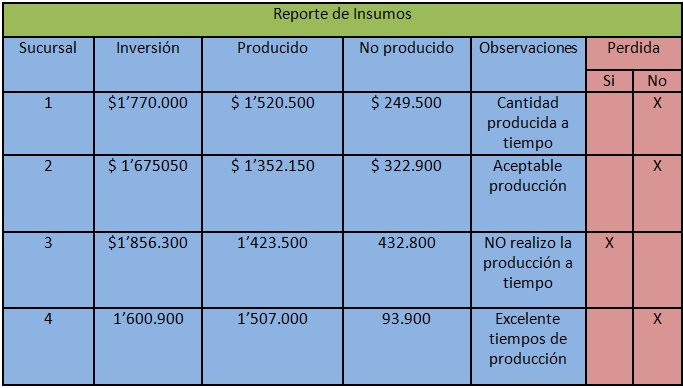
\includegraphics[width=0.60\textwidth]{images/REPORTEDEINSUMO.jpg}
%el caption es para el texto que aparece debajo de la imagen
	\caption{Reporte de insumo}
%label es para darle una referencia, por ejemplo si uno dice "como se puede ver en la imagen a1"
	\label{fig:Reporte de insumo}
\end{figure}%
\\%
\\%
\\%
\\%
\begin{figure}[htbp]
%centering es para centrar la imagen
	\centering
%aca es donde se incluye la imagen, se da el ancho(width), \textwidth significa que con repescto al tamano del
%texto y luego la ruta, relativa siempre es decir, a partir de donde se esta, como images esta ahi
%dentro, solo se usa desde images y ojala nada de espacios en el nombre de la imagen
		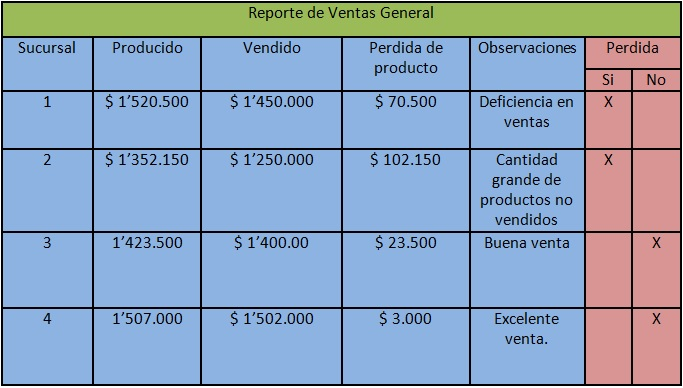
\includegraphics[width=0.60\textwidth]{images/REPORTEDEVENTASGENERAL.jpg}
%el caption es para el texto que aparece debajo de la imagen
	\caption{Reporte de ventas general}
%label es para darle una referencia, por ejemplo si uno dice "como se puede ver en la imagen a1"
	\label{fig:Reporte de ventas general}
\end{figure}%
\\%
\\%
\\%
\\%
\begin{figure}[htbp]
%centering es para centrar la imagen
	\centering
%aca es donde se incluye la imagen, se da el ancho(width), \textwidth significa que con repescto al tamano del
%texto y luego la ruta, relativa siempre es decir, a partir de donde se esta, como images esta ahi
%dentro, solo se usa desde images y ojala nada de espacios en el nombre de la imagen
		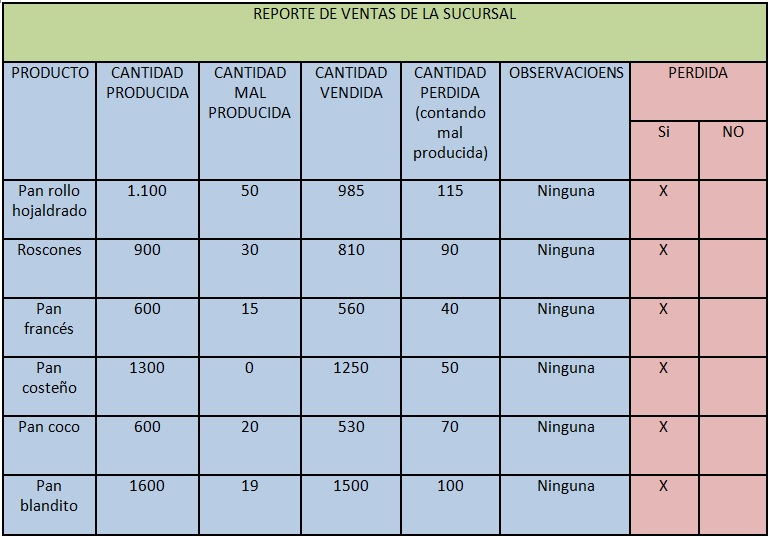
\includegraphics[width=0.60\textwidth]{images/REPORTEDEVENTASDELASUCURSAL.jpg}
%el caption es para el texto que aparece debajo de la imagen
	\caption{Reporte de ventas de una sucursal}
%label es para darle una referencia, por ejemplo si uno dice "como se puede ver en la imagen a1"
	\label{fig:Reporte de ventas de una sucursal}
\end{figure}%
\newpage%
\section{Dise\~no de interface}
Como primera medida notamos el ingreso al men\'u de sesiones donde se autorizara la gesti\'on de perfiles, teniendo en cuenta el nivel de seguridad pues la informaci\'on all\'i almacenada no es de uso p\'ublico.
\\%
Veremos inicialmente esta ventana:
\begin{figure}[htbp]
%centering es para centrar la imagen
	\centering
%aca es donde se incluye la imagen, se da el ancho(width), \textwidth significa que con repescto al tamano del
%texto y luego la ruta, relativa siempre es decir, a partir de donde se esta, como images esta ahi
%dentro, solo se usa desde images y ojala nada de espacios en el nombre de la imagen
		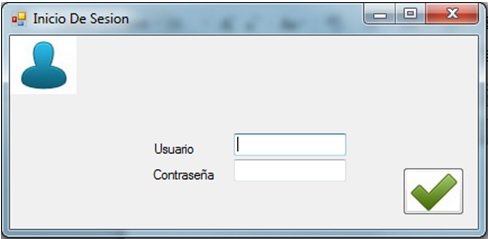
\includegraphics[width=0.60\textwidth]{images/Iniciosecion.jpg}
%el caption es para el texto que aparece debajo de la imagen
	\caption{Inicio de secion}
%label es para darle una referencia, por ejemplo si uno dice "como se puede ver en la imagen a1"
	\label{fig:Inicio de secion}
\end{figure}%
\\%
En el que evaluara que el Usuario y la Contrase\~na sean las correctas, a partir de esto el programa se encargara que opciones del men\'u le permita manipular.
\\%
\\%
Seguido a esto despu\'es de validar las contrase\~nas ofrecer\'a el siguiente men\'u:
\\%
\\%
%
\begin{figure}[htbp]
%centering es para centrar la imagen
	\centering
%aca es donde se incluye la imagen, se da el ancho(width), \textwidth significa que con repescto al tamano del
%texto y luego la ruta, relativa siempre es decir, a partir de donde se esta, como images esta ahi
%dentro, solo se usa desde images y ojala nada de espacios en el nombre de la imagen
		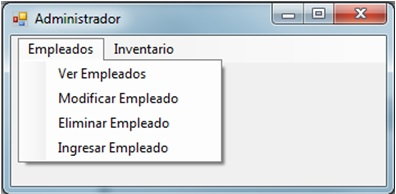
\includegraphics[width=0.60\textwidth]{images/Administrador.jpg}
%el caption es para el texto que aparece debajo de la imagen
	\caption{Ventana administrador}
%label es para darle una referencia, por ejemplo si uno dice "como se puede ver en la imagen a1"
	\label{fig:Ventana administrador}
\end{figure}%
\\%
\\%
En este despliegue de men\'u se seleccionara el procedimiento solicitado relacionado a los empleados.
\\%
\\%
\begin{figure}[htbp]
%centering es para centrar la imagen
	\centering
%aca es donde se incluye la imagen, se da el ancho(width), \textwidth significa que con repescto al tamano del
%texto y luego la ruta, relativa siempre es decir, a partir de donde se esta, como images esta ahi
%dentro, solo se usa desde images y ojala nada de espacios en el nombre de la imagen
		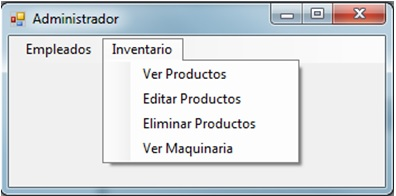
\includegraphics[width=0.60\textwidth]{images/Segundoadministrador.jpg}
%el caption es para el texto que aparece debajo de la imagen
	\caption{Ventana administrador}
%label es para darle una referencia, por ejemplo si uno dice "como se puede ver en la imagen a1"
	\label{fig:Ventana administrador}
\end{figure}%
\\%
\\%
En este despliegue de men\'u se seleccionara el procedimiento solicitado referente al inventario.
\\%
\\%
\begin{figure}[htbp]
%centering es para centrar la imagen
	\centering
%aca es donde se incluye la imagen, se da el ancho(width), \textwidth significa que con repescto al tamano del
%texto y luego la ruta, relativa siempre es decir, a partir de donde se esta, como images esta ahi
%dentro, solo se usa desde images y ojala nada de espacios en el nombre de la imagen
		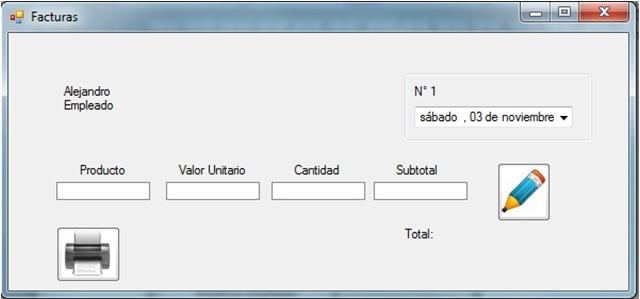
\includegraphics[width=0.60\textwidth]{images/Facturas.jpg}
%el caption es para el texto que aparece debajo de la imagen
	\caption{Ventana factura}
%label es para darle una referencia, por ejemplo si uno dice "como se puede ver en la imagen a1"
	\label{fig:Ventana factura}
\end{figure}%
\\%
\\%
Este men\'u se prioriza para realizar las facturas, con el fin de solicitar informaci\'on pertinente que sea necesaria.
\\%
\\%
\mbox{}
\newpage%
%
\mbox{}
\newpage%
%
\section{Recursos}
%
\mbox{}
\newpage%
\mbox{}
\newpage%
\mbox{}
\newpage%
\mbox{}
\newpage%
\section{Presupuesto}
%
\mbox{}
\newpage%
%
\mbox{}
\newpage%
%
\section{Cronograma}
%
\mbox{}
\newpage%
\mbox{}
\newpage%
\mbox{}
\newpage%
\mbox{}
\newpage%